\documentclass[12pt,a4paper]{article}
\usepackage{times}
\usepackage{durhampaper}
\usepackage{harvard}
\usepackage{graphicx}
\usepackage{algpseudocode}
\usepackage{algorithm}
\usepackage{subcaption}
\usepackage{caption}
\citationmode{abbr}
\bibliographystyle{agsm}

\title{User Interaction Discovery in Virtual Environments}
\student{L. A. Sutton}
\supervisor{W. Li}
\degree{BSc. Natural Sciences}

\date{\today}

\begin{document}

\maketitle

\begin{abstract}

{\bf Context/Background}

{\bf Aims}

{\bf Method}

{\bf Results}

{\bf Conclusions}

\end{abstract}

\begin{keywords}
user interaction; virtual environments; visualisation; clustering
\end{keywords}

\section{Introduction}

In the 21st century, people spend more time than ever interacting in virtual environments, whether that takes the form of social networking, email or video games. Many previous attempts have been made to visualise the structures that form within these environments \cite{freeman2000visualizing}

In this project I have taken 'User Interaction' to mean any way in which users consciously affect other users so that the other users would be able to identify the specific other users they were interacting with. This could take place over a period of time of be instantaneous; it could be between two users or many; it could be a single event or it could be ongoing. For example I will consider interactions such as users sending emails between one another but I will not consider interactions such as a user's advertising preference changing what another user sees as this falls beyond the scope I have layed out.

Virtual environments in this project will mean any environment in which users are able to interact in the ways I have previously mentioned, mediated by computers. This could be for example a video game, a social networking website or a messaging system such as email.

\subsection{Project Motivation}

While there have been many previous attempts to visualise the structure of virtual environments, these have almost exclusively focused on static representations of the relationships between users. From this a lot of data has been gathered about information presentation.

As has been seen, much of the previous efforts at visualisation and presentation had focused on the static representation of relationships between people in virtual environments. I wanted to extend this in two ways.

Firstly I wanted to extend the existing work that covered these static representations of relationships and take what was learned to apply to dynamic systems of interactions that were able to evolve over time.

Secondly I wanted to move the focus of the systems away from the current system of representing only the relationships between users that are inferred from the interactions. I would instead represent the interactions themselves.

\subsection{Project Aims}

These are the aims as laid out in my Design Report

\begin{enumerate}
\item Basic Deliverables
\begin{enumerate}
\item Develop a simple system that models user interactions with a visual output
\item Use this system to implement an existing model of user interaction
\item Expand this system and model to be able to visualise different modes of interaction
\end{enumerate}
\item Intermediate Deliverables
\begin{enumerate}
\item Expand the initial system so that its state will evolve over time according to the interactions of its users
\item Examine and visualise the way in which users cluster according to their interactions
\item Allow the system to set its initial state by real-world social network data
\end{enumerate}
\item Advanced Deliverables
\begin{enumerate}
\item Visualise change in the clustering of users according to their interactions over time
\item Generate quantitative output related to the change in clustering of users over time
\item Apply my quantitative output to attempt to solve a real-world problem
\end{enumerate}
\end{enumerate}

\section{Related Work}

\subsection{Social Network Visualisation}
Network visualisation is already a science with a long history, especially since being able to use computers to position and draw the output. There are currently low-level tools that exist with the intention that they have the necessary flexibility to accommodate a wide variety of visualisation styles and techniques \cite{heer2005prefuse}. As well as this, there are tools that exist to provide numerical analysis \cite{borgatti2002ucinet}. However, these tools have focused on the analysis and visualisation of snapshots of data remaining static, rather than data sets that evolve over time. These have also previously been used to build ways of visualising social network data from Friendster \cite{heer2005vizster} in order to facilitate discovery of more information than would be apparent from other ways of looking the data, as I hope to.

\subsection{Information Presentation}
There is also a wide variety of information on the presentation of data on computer screens. One particularly popular model can be summed up as 'Overview, Zoom, Filter' \cite{shneiderman1996eyes}. In this it is suggested that the initial view of the data should be a movable field of view with emphasis on allowing the user to gain an 'overview' of relevant data and identify areas which will be of interest. Specific areas of interest can then be zoomed in on preserving the context of the overall picture before extra information of areas of interest can be viewed possibly by clicking on them. This paper also talks about things such as the importance of smooth display updates and responsiveness to user input. This is built upon by the ideas of making information more clear by distorting the 'presentation space' \cite{carpendale2001framework}. This is the method used in Vizster and can be seen in common usage in many different data visualisation applications. It imagines that the virtual space in which the data is presented is a real material that can be stretched and viewed through a movable lens as necessary to make the relevant areas of the information more clear. These ideas area also expanded on further to see what kinds of lenses are suitable for which purposes, and suggests a mathematical framework for implementing such a lens \cite{leung1994review}. Contained in all of these articles on visualisation are also many suggestions for evaluation of data presentation on computers for example by the ability to maintain context between switching between the three areas on the 'Overview, Zoom, Filter' model and the responsiveness to user input that is possible.

\subsection{Graph Drawing}
There is also previous literature on the drawing of graphs in aesthetically pleasing ways. Almost all current research makes use of a force directed spring layout. In this algorithm, each node is modelled is repelling each other node and the edges between them are modelled as springs\cite{fruchterman1991graph}. Included in these papers are suggestions for the strength of the attractive and repulsive forces different distances and the size of graph that this can be expected to create. However, this algorithm doesn't scale well with rapidly increasing numbers of vertices. It has been pointed out that with a large number of nodes, calculating the layout in this way is very expensive in terms of computing power. However, with the correct optimisations it is possible to reduce the complexity to $o(nlog(n))$ \cite{barnes1986hierarchical}.

\subsection{Modelling Social Networks}
The ability to produce networks of relations and interactions from many different data sources is also explored in a variety of different papers. For example, networks of social interaction have been produced from a history of email correspondence within an organisation \cite{fisher2004social}. Here other relevant ideas are explored such as the privacy implications of collecting data on a large scale and the ability to reconstruct the whole graph from only partial data. The same has also been achieved using the transcript of an internet relay chat \cite{mutton2004inferring} again struggling with the problem of reconstructing a complete graph from partial data. It is then further shown that the same method including the temporal decay of relationships can be applied to other sources of relationship information involving over time such as the plays of William Shakespeare.

\subsection{Categorisation of Interactions}
Previous reserach has also explored categorisation of interactions by their characteristics. This has mainly in the past been applied to social iterations writing 3D virtual environments in which people interact as virtual avatars, referred to as Networked-Virtual Environments. One particular application of this is games \cite{manninen2000interaction}. Here we can see that there is more than one way of categorising interactions, one way being based on their purpose. These papers also show how it is possible for many different modes of interaction to happen simultaneously. It is possible to use communicative action theory to categorise interactions by their purpose, this is extended in other papers by comparing interactions in a selection of game environments \cite{becker2002social}. Extending this to other environments such as the social network, other papers show how much of the interaction that goes on writhing a virtual environment is hidden from the user. We can see just how much data website such as Facebook collect about us including in our making interactions which we wouldn't normally consider meaningful \cite{schneier2010taxonomy}

\subsection{Evolution of social networks}
Ideas of the behaviour of users in social networks have been the subject of many different papers. This includes homophily \cite{adamic2003social} which is the idea that people on social networks tend to associate with people who are similar to themselves in terms of age, political views etc. Work has also been completed on the behaviours of users within a social network and the ways in which interactions can spread behaviour across networks of people represented as graphs. It has been suggested that this can be explained using a virus like model \cite{centola2010spread} in which users pass between susceptible, infected and recovered states, analogous to a computer-virus or a real virus.

\subsection{Detection of clustering}
Detecting features of social networks that are not immediately apparent is also extremely important. We can see that algorithms have been developed that aim to detect communities, related to clustered sections of graph representations of these networks \cite{newman2004fast}. These algorithms can be applied to real world networks with a good degree of success reported in identifying the same communities that the users themselves identify with.

\section{Solution}

My solution focuses on flexibility and allows the user to enable and disable as well as configure many different elements. These various elements are described below.

\begin{figure}[htb]
\centering
\caption{Architectural diagram of solution}
\label{fig:diagram}
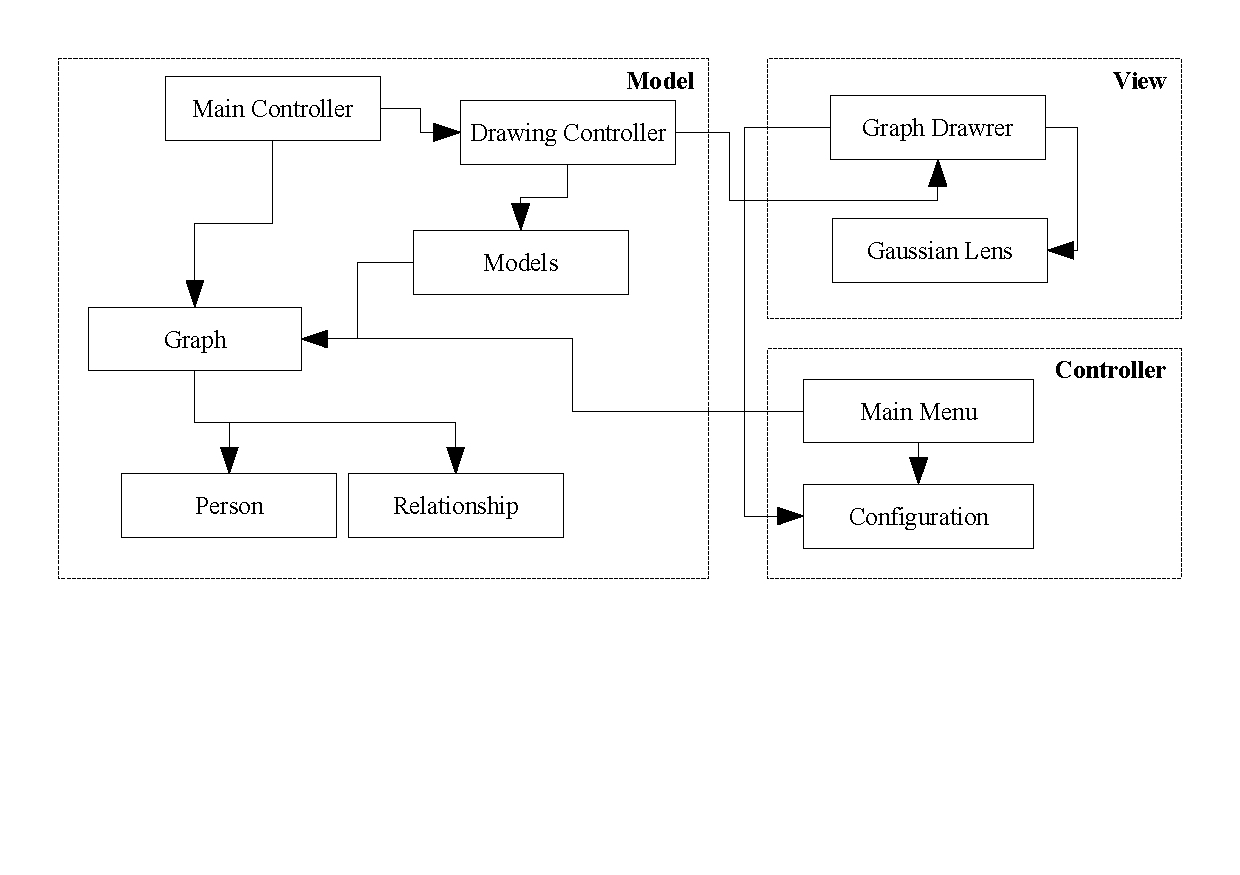
\includegraphics[scale=0.75]{ArchitectureDiagram.pdf}
\end{figure}

The implementation roughly followed a model, view, controller design pattern in order to ensure that the elements remained as separate as possible

\subsection{Menu System}

The primary control of the system is given initially though a system of menus which are presented to the user before the system begins running.

\begin{figure}[htb]
\centering
\caption{Example menu system of the solution}
\label{fig:menu}
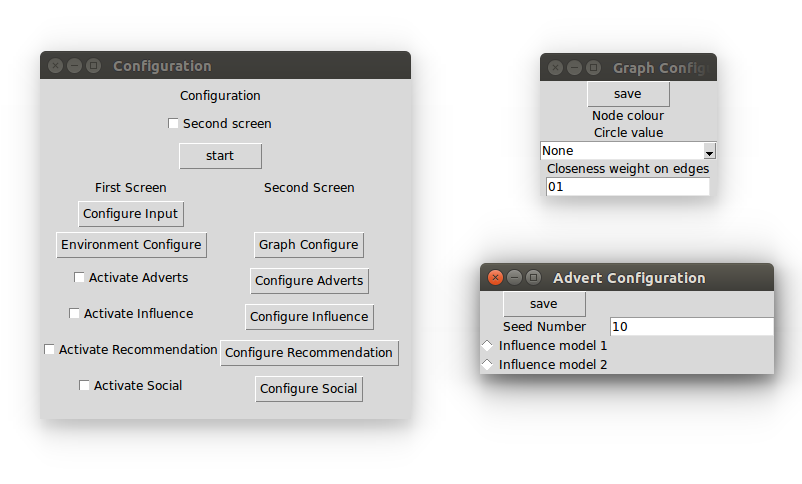
\includegraphics[scale=0.5]{MenuShot.png}
\end{figure}

Figure \ref{fig:menu} shows an example of these menus. The main window on the left represents the main control of the application. In this window it is possible to enable and disable the various demonstration models that can be used in order to demonstrate the visualisation system. The buttons next to these check boxes allow various aspects of each the demonstration to be configured so as to give different results. The aspects that can be configured are detailed in the descriptions of each system below.

This menu also allows the user to select what initial input data will be used. They can either generate random data that will be realistic enough in order to demonstrate the system or import their own data. Users own data must come from the netvizz Facebook app (https://apps.facebook.com/netvizz). This allows users to download a 'gml' file containing a list of all friends of a user, the sex of the users, how many things they like and a seperate list of all friendships between the listed users in order to build up a network.

\subsection{Interactions with Vertices}

The user is able to interact with vertices representing people in the graph in two different ways. These are shown in \ref{fig:labels}.

\begin{figure}[htb]
\centering
\caption{Diagram showing labels and selctions}
\label{fig:labels}
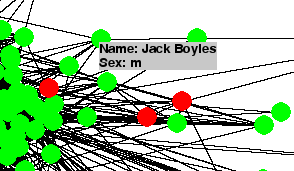
\includegraphics[scale=1]{Select.png}
\end{figure}

The first way is that if the user has selected it as an option in the first menu, they have the ability to move their mouse over a node in order to see more information about it. This can be seen as the box with a grey background in the figure. It can be configured to show what information the user requests, in this case it shows the name and sex of the person represented by the vertex.

The second way in which the user can interact directly with vertices is by clicking on them. This has a different meaning depending on the context for example, it could be used to select the points being used to seed in the advert or influence models laid out below. This would work as in the picture if say, a user was to select a green vertex it would change colour to indicate it was selected and if a user selected a red vertex it would change back to green in order to indicate it was deselected.

\subsection{Graph Layout}

This element of my solution is always enabled and allows the system to draw its main view which is a representation of the relationships between the people interacting at that moment. The system that I have used to lay out my graph has been taken form \cite{fruchterman1991graph}.

Current data visualisations make almost exclusive use of a force-directed spring layout for graph drawing. This method models a graph as a set of springs along each edge joined at each node. These springs, as in my case, need not respond to force in the same way as a real, physical spring but can instead have whatever response gives the best layout for the graph.

The algorithm can then use an iterative approach in order to find a local point of least tension on the springs as a collection. 

\begin{algorithm}[htb]
\caption{Graph sprint-directed layout algorithm}
\label{alg:graph}
\begin{algorithmic}
\State $graph \gets (V, E)$ \Comment{Graph represented as a collection of vertices and edges}
\State $k \gets \sqrt{1/|V|}$
\State $t \gets 0.05$
\ForAll{Vertex in V}
	\State $Vertex.displacement \gets (0,0)$
	\ForAll{Other in V \textbackslash Vertex}
		\State $dist \gets distance(Vertex, Other)$ \Comment{$distance$ gets Euclidean distance}
		\State $diff \gets (Vertex.x-Other.x, Vertex.y-Other.y)$
		\State $Vertex.displacement \gets Vertex.displacement + diff \times (k^{2}/dist)$
	\EndFor
\EndFor
\ForAll{Edge in E} \Comment{Edge between two vertices, $V_{1}$ and $V_{2}$}
	\State $dist \gets distance(V_{1}, V_{2})$
	\State $diff \gets (V_{1}.x-V_{2}.x, V_{1}.y-V_{2}.y)$
	\State $V_{0}.displacement \gets V_{0}.displacement - diff \times (dist^{2}/2k)$
	\State $V_{1}.displacement \gets V_{1}.displacement + diff \times (dist^{2}/2k)$
\EndFor
\ForAll{Vertex in V}
	\State $(Vertex.x, Vertex.y) \gets (Vertex.x, Vertex.y) + (Vertex.displacement/distance(Vertex.displacement)) \times (min(distance(Vertex.displacement), t))$ \Comment{$min$ gives minimum of two elements}
	\State $(Vertex.x, Vertex.y) \gets min(0.95, max((Vertex.x, Vertex.y), 0.05))$ \Comment{$max$ gives maximum of two elements}
\EndFor
\end{algorithmic}
\end{algorithm}

\begin{figure}[htb]
\caption{Graph Layout}
\label{fig:layout}
\centering
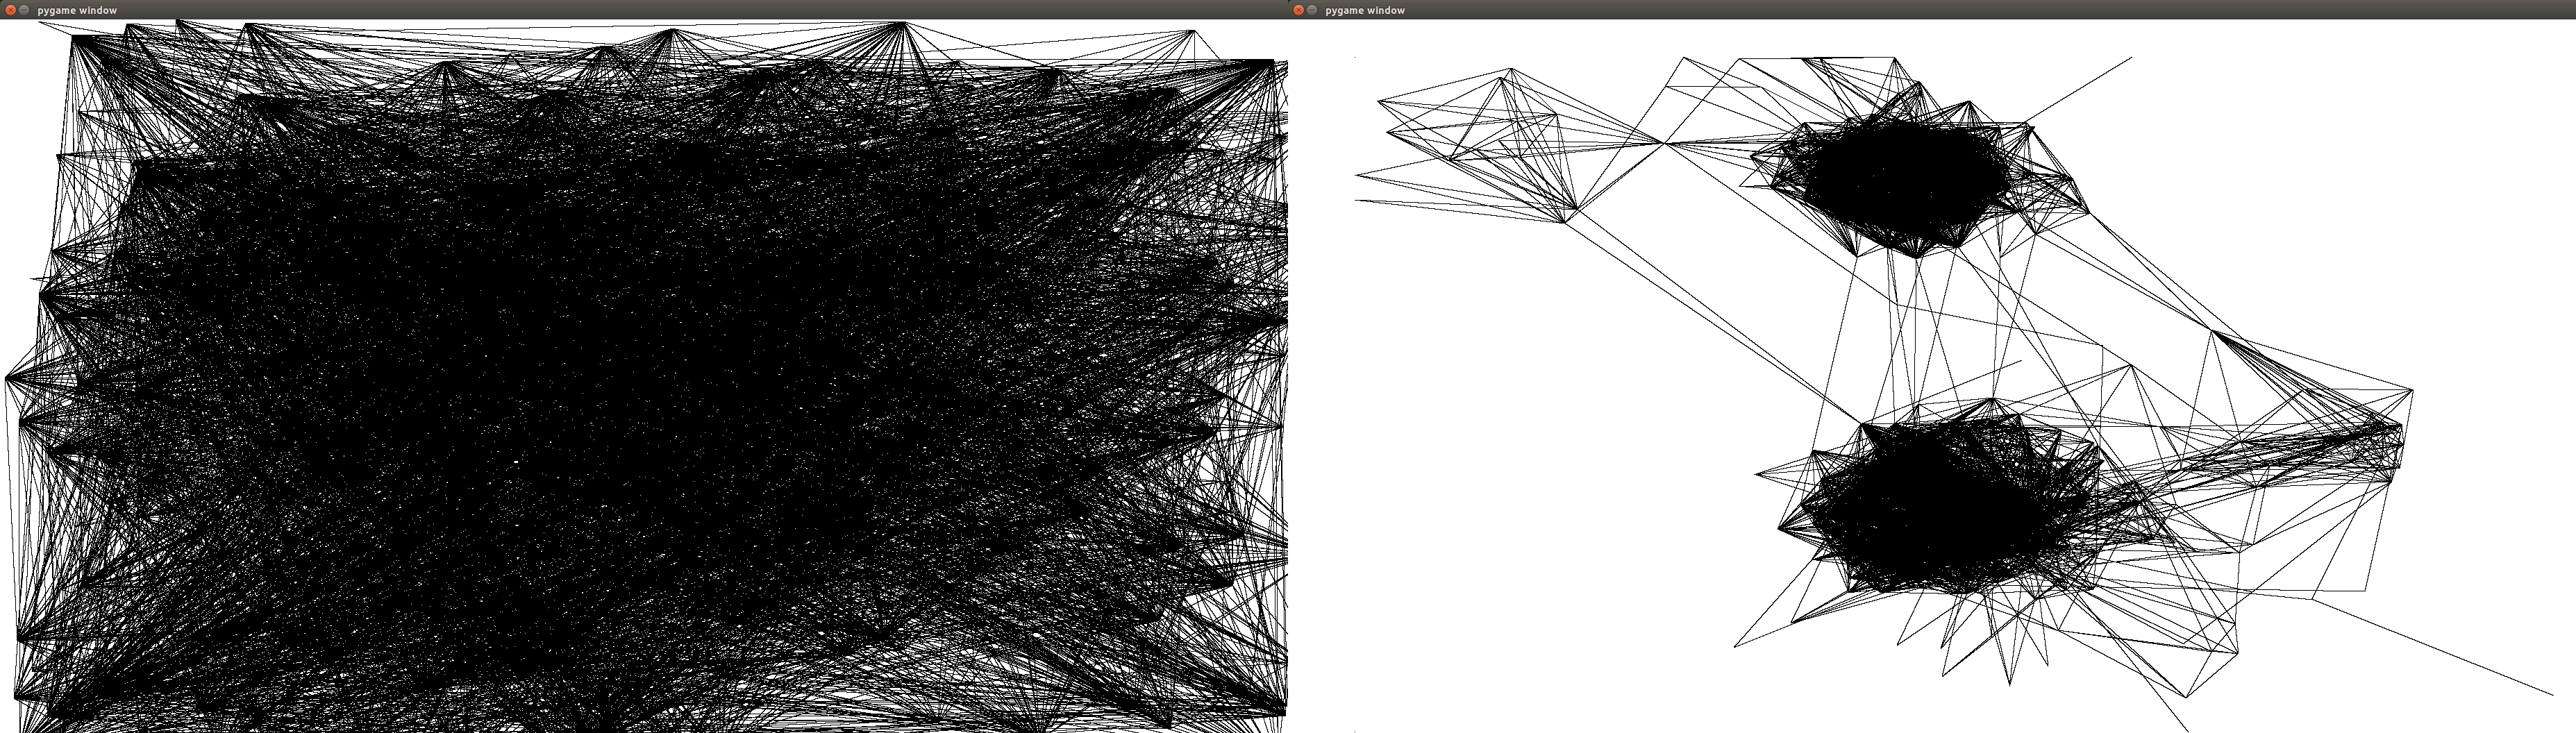
\includegraphics[scale=0.12]{Pygame.png}
\end{figure}

I have detailed the algorithm that I used in Algorithm \ref{alg:graph}. This is split into three main parts after the set up. Initially the value of $k$ is set to the value suggested in the above paper and $t$ is set to a value which was determined through testing to be the best.

Ever vertex starts with 0 displacement. The first part of the algorithm then calculates the repulsion between every pair of vertices and updates its displacement an amount proportional to the inverse of the distance. The second part of the algorithm then calculates the attraction along every edge and updates the displacement of each vertices in this edge proportionally to the square of the distance. Finally, each vertex is moved either its displacement or t, a pre-determined distance, whichever is smaller, then the algorithm checks that none of the points have been moved outside the boundary of the screen.

In my implementation, the input graph is initially laid out totally at random. We can then see an example of an application of this algorithm over a number of iterations in figure \ref{fig:layout}. It can be seen how the points are taken from a random layout to a layout in which it is easy to see the structure of the graph.

\subsection{Lens}

Many of these layouts, especially since they include a large number of points in a small area can become hidden. After experimentation it was decided that a Gaussian lens would be best suited for this. This was mainly because of the gentle falloff and smooth transition through the point of maximum focus that made the interaction natural as the user moved the 'lens' around the visualisation.

\begin{equation}
\label{eq:Guass}
f(x,\mu,\sigma)=\frac{1}{\sigma\sqrt{2\pi}}e^{\frac{(x-\mu)^{2}}{2\sigma^{2}}}
\end{equation}

A Gaussian distribution is given by equation \ref{eq:Guass}. In my solution $f(x, \mu, \sigma)$ represents the distance that the point will be displaced away form the cursor. In my implementation $x-\mu$ is the initial distance between the vertex and the cursor and $\sigma$ is a value that was determined by experiment in order to give the best result. I settled on 0.1, meaning that vertices over 20\% of the width or height of the screen away would no longer be significantly affected.

\begin{figure}[htb]
\caption{Example of lens}
\label{fig:lens}
\centering
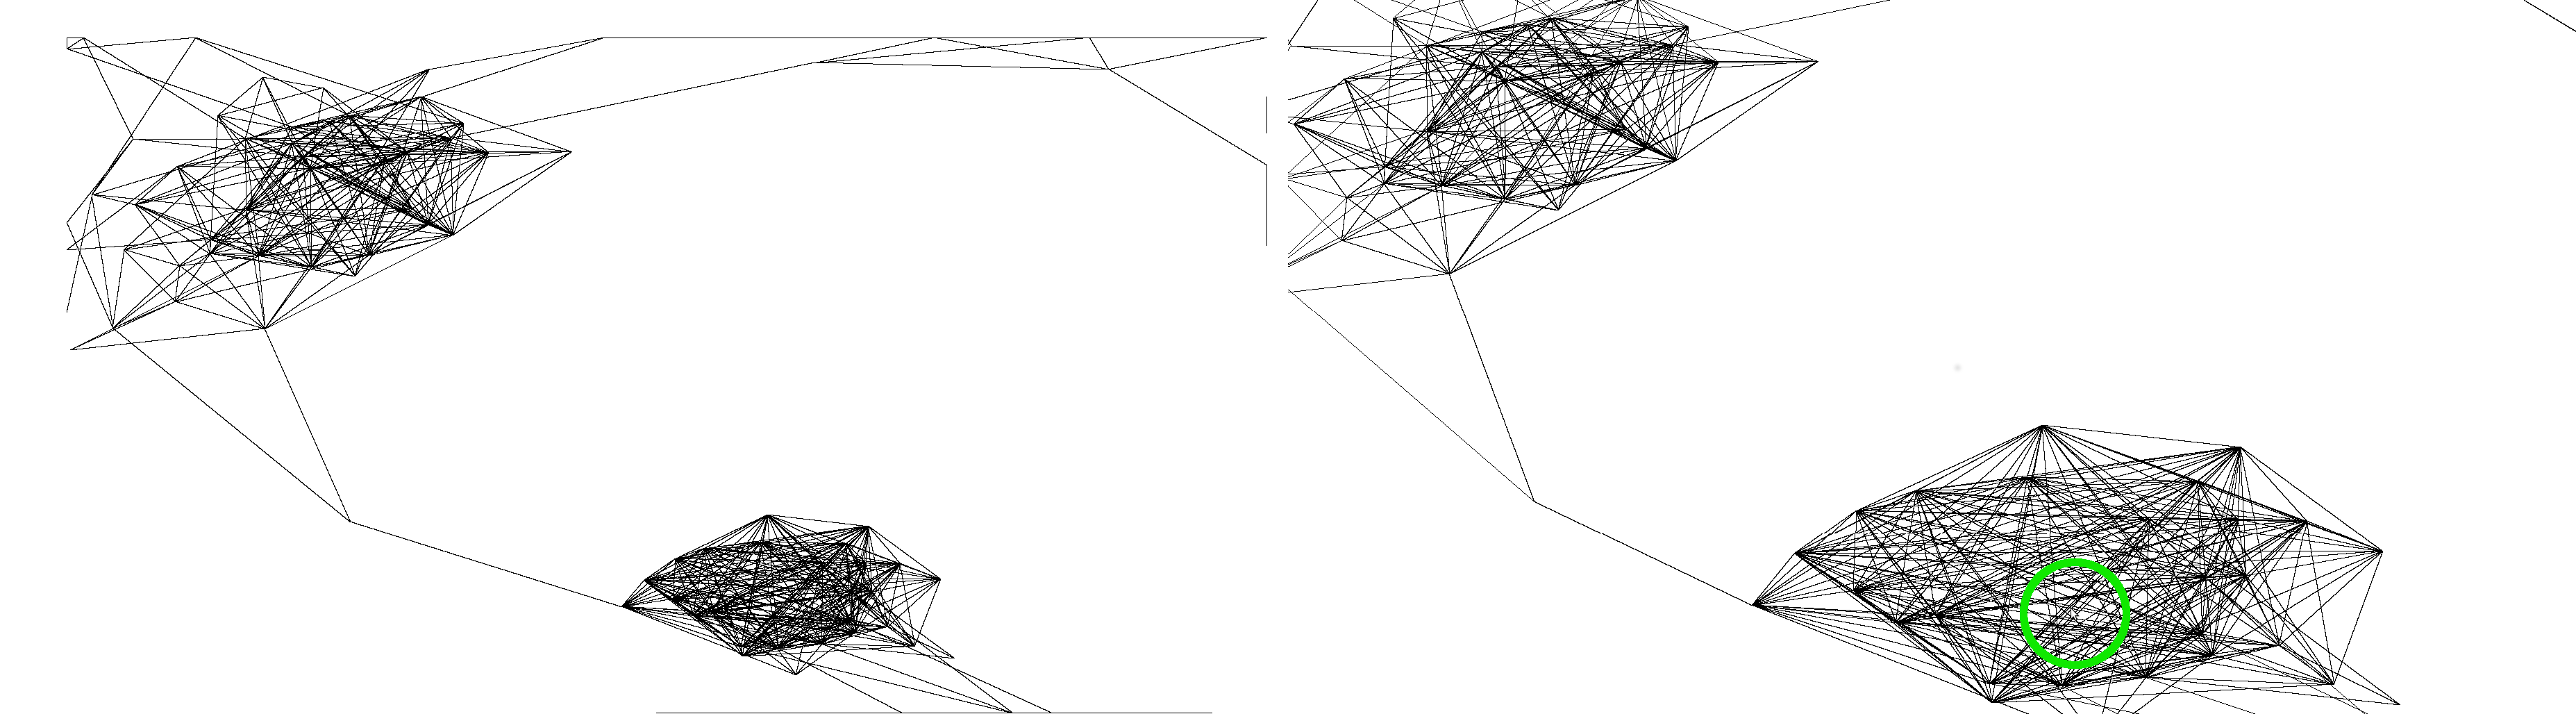
\includegraphics[scale=0.12]{Gaussian.png}
\end{figure}

It can be seen in figure \ref{fig:lens} that the lens allows the interactions surrounding the cursor (highlighted by a black ring) to be viewed much more effectively.

\subsection{Transitions}

One way of showing interactions between users in real times is by showing movement in the graph. An example of this can be seen in figure \ref{fig:transitions}. In this case these are being used to show the likes that users give others in the 'social' demonstration laid out below. As a user likes another's post a Facebook 'thumb' image is generated at the person who likes and travels over the course of about a second to the person who's post is being liked.

It is possible to use this as well to represent other interactions such as the spread of influence. The 'thumb' can be replaced by another image or by a simple disc or other relevant symbol.

\begin{figure}[htb]
\caption{Examples of transitions}
\label{fig:transitions}
\centering
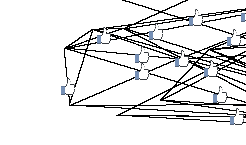
\includegraphics[scale=1]{Transitions.png}
\end{figure}

\subsection{History}

In order to make a fast moving interaction more clear, it is possible for the system to record the state of each user at given times and then to display this data once the model has run.

\begin{figure}[htb]
\caption{Example if a display of the history of states}
\label{fig:history}
\centering
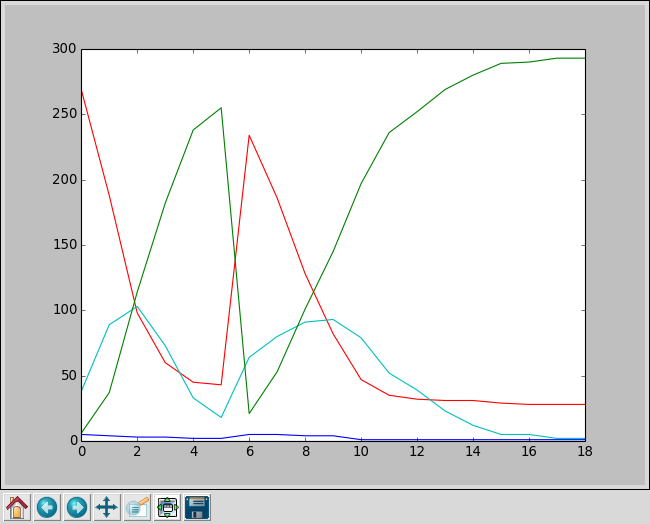
\includegraphics[scale=0.3]{Graph.png}
\end{figure}

An example of this can be seen in figure \ref{fig:history}. In this case the history is taken from an example running of the viral advertising model detailed below. The horizontal axis represents time while the vertical axis represents the number of users. In this case the colours in the graph match the colours that are used to represent the vertices in the graph view.

This visualisation makes it clear how the distribution of users changed over time. In this view the progress of the first campaign can clearly be seen, as can the jump when this campaign is ended and a second introduced.

\subsection{Vertices}

The system allows for many different ways of representing people as vertices depending on their attributes in order to make it as clear as possible what is being represented.

\begin{figure}[htb]
\caption{Examples of possible representations of vertices}
\label{fig:vertices}
\centering
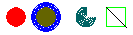
\includegraphics[scale=1]{Nodes.png}
\end{figure}

Figure \ref{fig:vertices} shows examples of different ways that attributes of the vertex can be changed in order to show different information.

The vertex on the left represents the most basic at only one solid colour, this colour could change for example to represent changes of state between a finite number of states or could have its brightness or hue changed to represent a continuous change in a property. For example in the advertising system detailed below the vertex changes colour to indicate what stage it has reached in the viral campaign.

The second vertex from the left shows that this can be build up in layers with an edge or another band of colour. This could be used to represent multiple properties win the same vertex. For example if the user wanted to track the difference that starting variables made to a system or to run multiple systems simultaneously that all relied on being represented by colour change of the vertex.

The second vertex from the right shows how it is then further possible to represent properties by the length of a filled arc around a vertex. This could be used to represent the state of a property that it is known will fall between two bounds for example age.

The final example on the far fight shows how it is possible to represent vertices as arbitrary shapes constructed as necessary in order to be fully customisable for whatever is being represented at the time.

\subsection{Edges}

There are multiple ways of using edges of the graphs to represent the relationships between people. A selection of these can be seen in figure \ref{fig:edges}.

\begin{figure}
\caption{Examples of possible representations of edges}
\label{fig:edges}
\centering
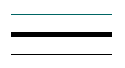
\includegraphics[scale=1]{Edges.png}
\end{figure}

The bottom line shows how edges are generally represented as a single pixel line joining the two users who have a relationship between then.

The middle like then shows that the thickness of the line can be changed in represent different things about the relationship between two people. This could for example be used to represent the strength of the relationship between two people.

Finally I have shown how it is possible to change the colour of the line joining the two vertices. This could be changed to represent some interaction between he users and can obviously be combined with either of the two previous methods.

\subsection{Demonstration Models}

In my implementation I included a set of demonstrations in order to show off the usefulness and effectiveness of my implementation as applied to real-world scenarios.

\subsubsection{Influence}

I implemented the two models of influence spreading through a social network according to \cite{kempe2003maximizing}. This could be used to model behaviour adoption across a social network, for example if a new social game such as 'Farmville' were to be released, this could simulate how social network users would encourage their friends to also play the game.

In the first model of influence, based on 'Linear Threshold Model', initially each vertex is given an adopted value of $False$ a value representing the influence that they are currently feeling and an adoption value, representing how much influence must be exerted over them in order for them to adopt the behaviour. A given set of starting nodes are then chosen and have their adopted value set to $True$. The model then proceeds in steps. At each step, first the weights of all connections to that vertex are added up, then the weights of each vertex that has adopted the behaviour. If the weights of vertices that has adopted divided by the weights of all neighbour is greater than the vertices adoption value, that vertex then adopts the behaviour.

In the second model of influence based on the 'Independent Cascade Model'. Initially, similarly to before each vertex is given a property to show that it hasn't adopted the behaviour, and a random set are chosen to have adopted it. As before the model then proceeds in steps. In each step, each vertex that has adopted the behaviour will have one chance to influence its neighbours to adopt the behaviour. Whether or not they are successful depends both on the 'strength' of the edge between the two vertices and a random element. Each node that is successfully influenced has only one chance to influence its neighbours, but one node will have multiple chances to be influenced if it has multiple neighbours who are influenced.

In this model it is possible to configure many different aspects such as the number of starting nodes and the relative chances of the behaviour being adopted. It is also possible to use both models simultaneously in order to compare their results.

\subsubsection{Advertising}

I implemented a model of the spread of viral advertising within an online environment. This model was based on \cite{van2010viral} and relies on a transition of each person between a number of states. These states are: People who haven't participated in the campaign; people who have received a 'seed' email; people who have seen a traditional advert as part of the campaign;  people who have received an email from a friend about the campaign; people who have chosen not to participate and finally people who have participated.

In the initial setup, all vertices have a status set that they have not participated in the campaign. A random number of 'seed' emails are then sent to people, then a number of 'seed' adverts are shown to the vertices, again with a chance to trigger participation in the campaign. As before this campaign proceeds in steps. At each step, a certain number of vertices being considered will check their email. If they have received an email related to the campaign, either from another user or a 'seed' email then this will give them either a chance to participate in the campaign or choose not to. If they choose not to, nothing happens, if they choose to participate in the campaign, they will then generate emails to a random number of their friends about the campaign and the cycle continues.

In this case it is possible to change all of the relevant variables in order to see their effects such as the number of seed emails sent and the number of users initially seeing the seed advert. It is also possible to determine how likely a user is to respond to either an advert or an email or even to give different response rates for emails from their friends and seed emails.

\subsubsection{Recommendation}

I implemented a model such as might be found in a social recommendation system as inspired by \cite{walter2008model}. This model imagines a system in which users are recommended something, say, films according to what their friends report they enjoyed.

This system begins by seeding a number of ratings for a number of different items, ratings are a value between 0 and 1. Recommendations are then propagated through the graph. This happens once, each vertex looks through its neighbours to see if it can find someone who has a direct opinion of the product, if it fails to find anyone it then looks through its neighbours neighbours and so on until it either finds someone or reaches a pre-determined depth. If it does find somebody it then takes this recommendation with a degradation depending on how many edges separate the vertex under consideration and the one doing the recommending.

It is possible in this model to change several variables within the system such as the number of users that are initially seeded with experiences of what is being recommended, what experience these users have and the depth to which a user will search for a recommendation. This system also accommodates there being multiple items which can each have their own recommendations propagated on their own

\subsubsection{Social}

Finally I took a different approach and implemented a system of interactions such as might happen over a social network. For this I primarily used my personal experiences on Facebook, a platform that I use to interact with people online daily. It is difficult to find reliable statics to use in such a model but in the end I settled on a website which had correlated statistics from many sources of varying reliability \cite{facebookStats}. I was satisfied with this however as it was not necessary for my model to be perfect, only sufficiently accurate to show how my visualisation could be applied to a real situation.

The model encompasses various elements of the Facebook website. Each user has a wall on which they can post either a status of a picture at random intervals, pictures can have one or more friends tagged in them. Each user also has an attribute 'views'. Users will at random intervals check their news feed which is made up of posts from the walls of their friends. Their attitude towards their friends can change according to their attitude towards any other people that might appear tagged in pictures, or the difference in 'views' between a person reading a status and the person writing it.

\subsubsection{Tools Used}

The solution is entirely written using a combination of Python 3.4 and various libraries. I used a 64 bit binary of version 3.4.2 of CPython as my interpreter, downloaded from www.python.org. This was chosen as at the time of writing it was the latest version of the most popular Python interpreter. I used a 64 bit edition so that if it became necessary I would be able to make use of all available memory of my computer and python 3 was chosen rather than python 2 so that I was able to make use of recent performance optimisations.

Visualisations were produced using the PyGame library. I obtained this by building the source available from https://bitbucket.org/pygame/pygame on my system at the time of writing with CPython as mentioned above. PyGame was chosen because if its ease of use over OpenGL allowing for rapid prototyping. Additionally its use of optimised C code would ensure that the visualisations would not interfere with time required for other computations.

Menus were implemented in the solution using the Python package Tkinter. This was obtained from my system's package repository (http://archive.ubuntu.com/ubuntu/dists/utopic/). I chose to use this as it would provide easy implementation of menus in my solution while not distracting from the models being used.

Graph drawing was done using the pyplot library from Matplotlib. This was as with Tkinter obtained from by systems package repository. I chose this as a method of graph drawing as it provided easy drawing of simple graphs and would easily allow me to change the style in order to experiment with different ways of displaying the data.

\subsection{Verification and Validation}

Software verification was undertaken at all stages of the implementation. This was primarily achieved with reference to my Design Report, in which I had given thought to the design and architecture necessary in order to achieve the objectives set out at the beginning of the project.

Software validation was made in reference to the objectives and functional requirements set out in my Design Report which were designed to allow me to meet the objectives of the project in several layered steps. This was also helped by the project supervisor who advised on direction at all stages and ensured that focus was maintained on the areas in which it was most needed.

\subsection{Testing}

As I prototyped my implementation, I undertook both static and dynamic testing to ensure that my project was both valid and verified 

\section{Results}

In order to demonstrate my system I made serveral mock ups to show what it could be capable of. I present those here.

\subsection{Viral System}

Here I implemented the Viral model specified above.

\begin{figure}
\centering
	\begin{subfigure}[b]{0.3\linewidth}
	\caption{Viral graph view, showing the states of the people}
	\label{fig:viralStates}
	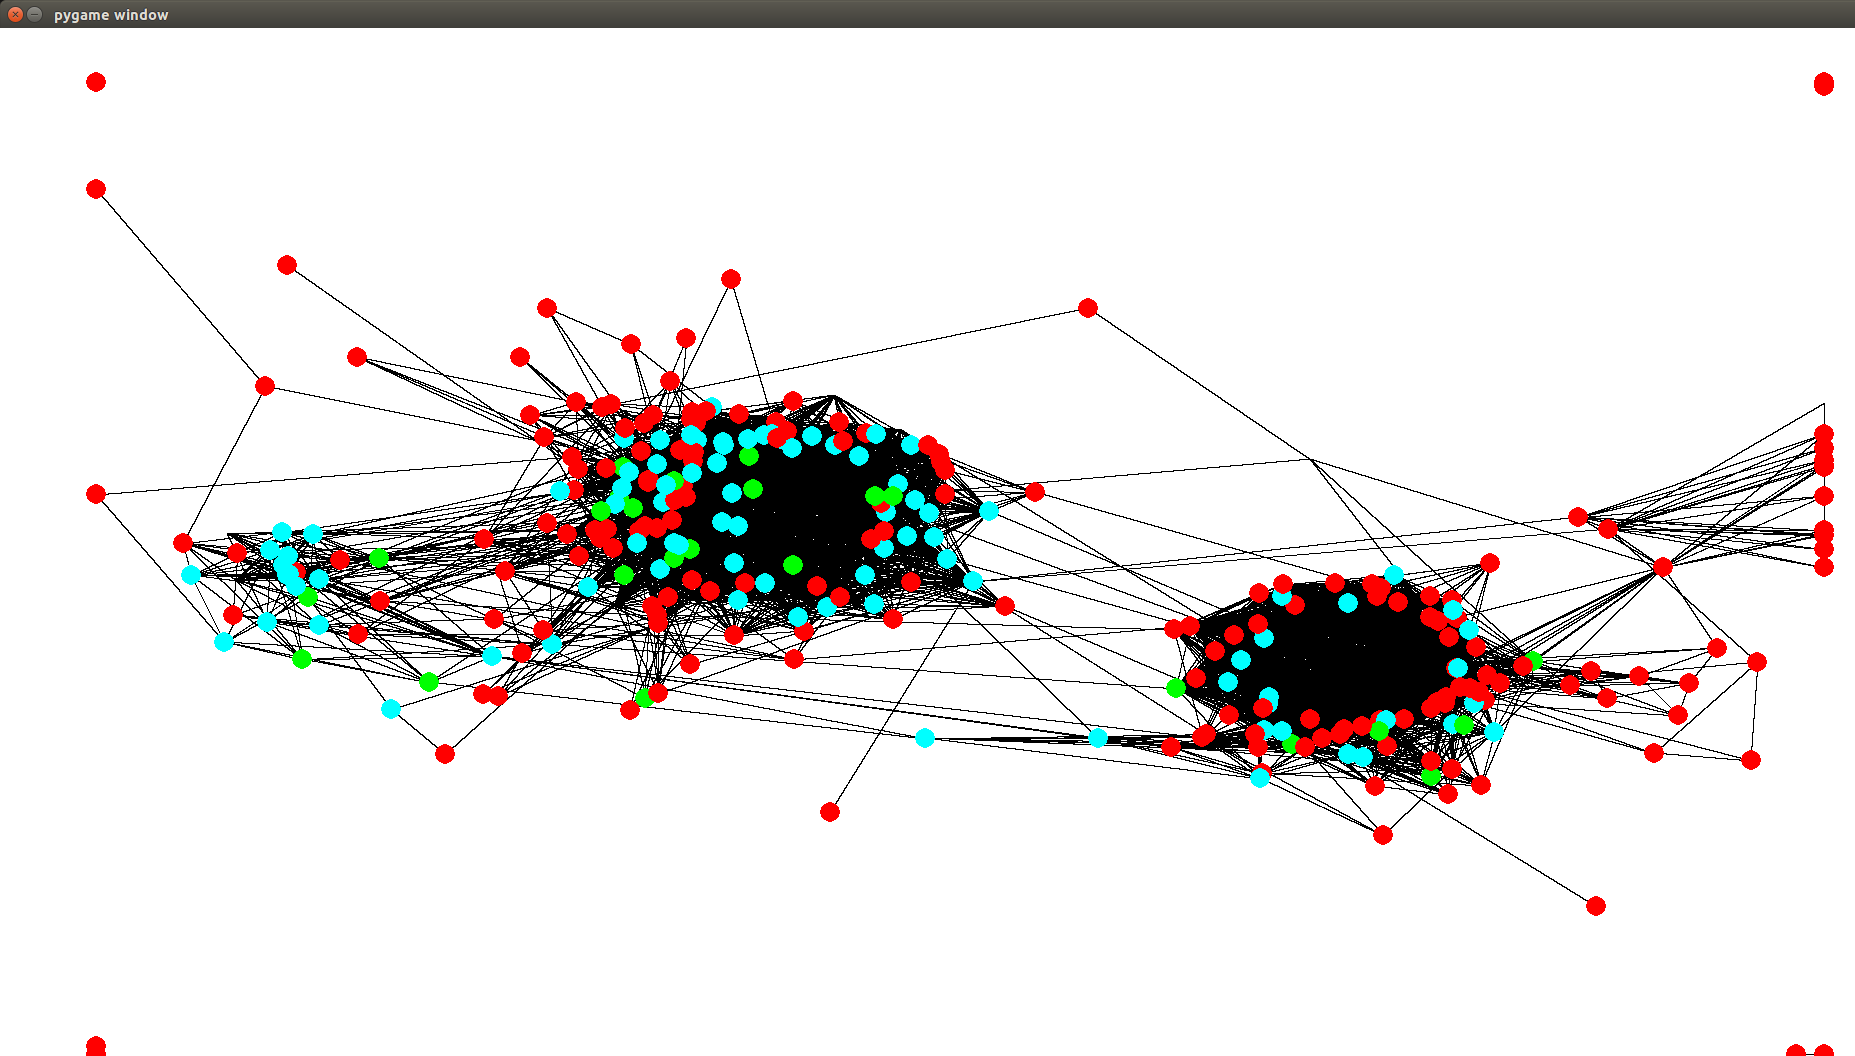
\includegraphics[scale=0.1]{Viral1.png}
	\end{subfigure}

	\begin{subfigure}[b]{0.3\linewidth}
	\caption{Window showing configuration of new viral campaign}
	\label{fig:viralConfig}
	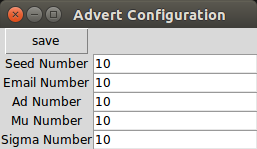
\includegraphics[scale=0.3]{Viral2.png}
	\end{subfigure}
\quad
	\begin{subfigure}[b]{0.3\linewidth}
	\caption{Graph showing evolution of states of people over time}
	\label{fig:viralGraph}
	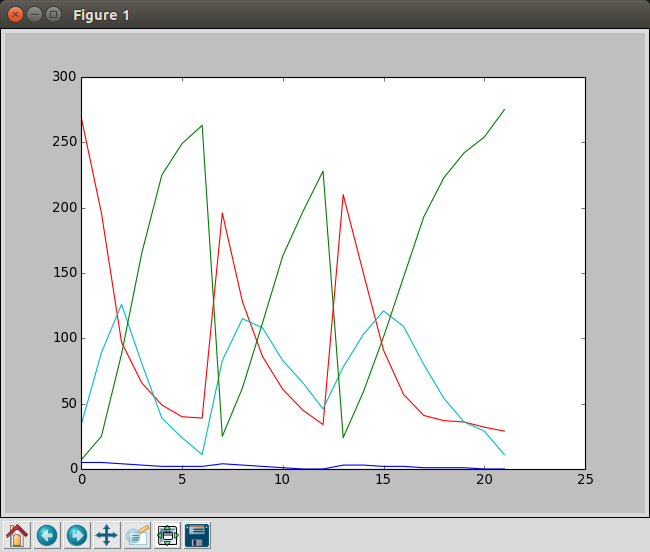
\includegraphics[scale=0.2]{Viral3.png}
	\end{subfigure}
\caption{Examples of output produced from Viral model}
\label{fig:viral}
\end{figure}

\subsection{Recommendation System}

\begin{figure}
\centering
	\begin{subfigure}[b]{0.4\linewidth}
	\caption{Initial graph view showing who has experienced and who has been recommended a product}
	\label{fig:recommendationInitial}
	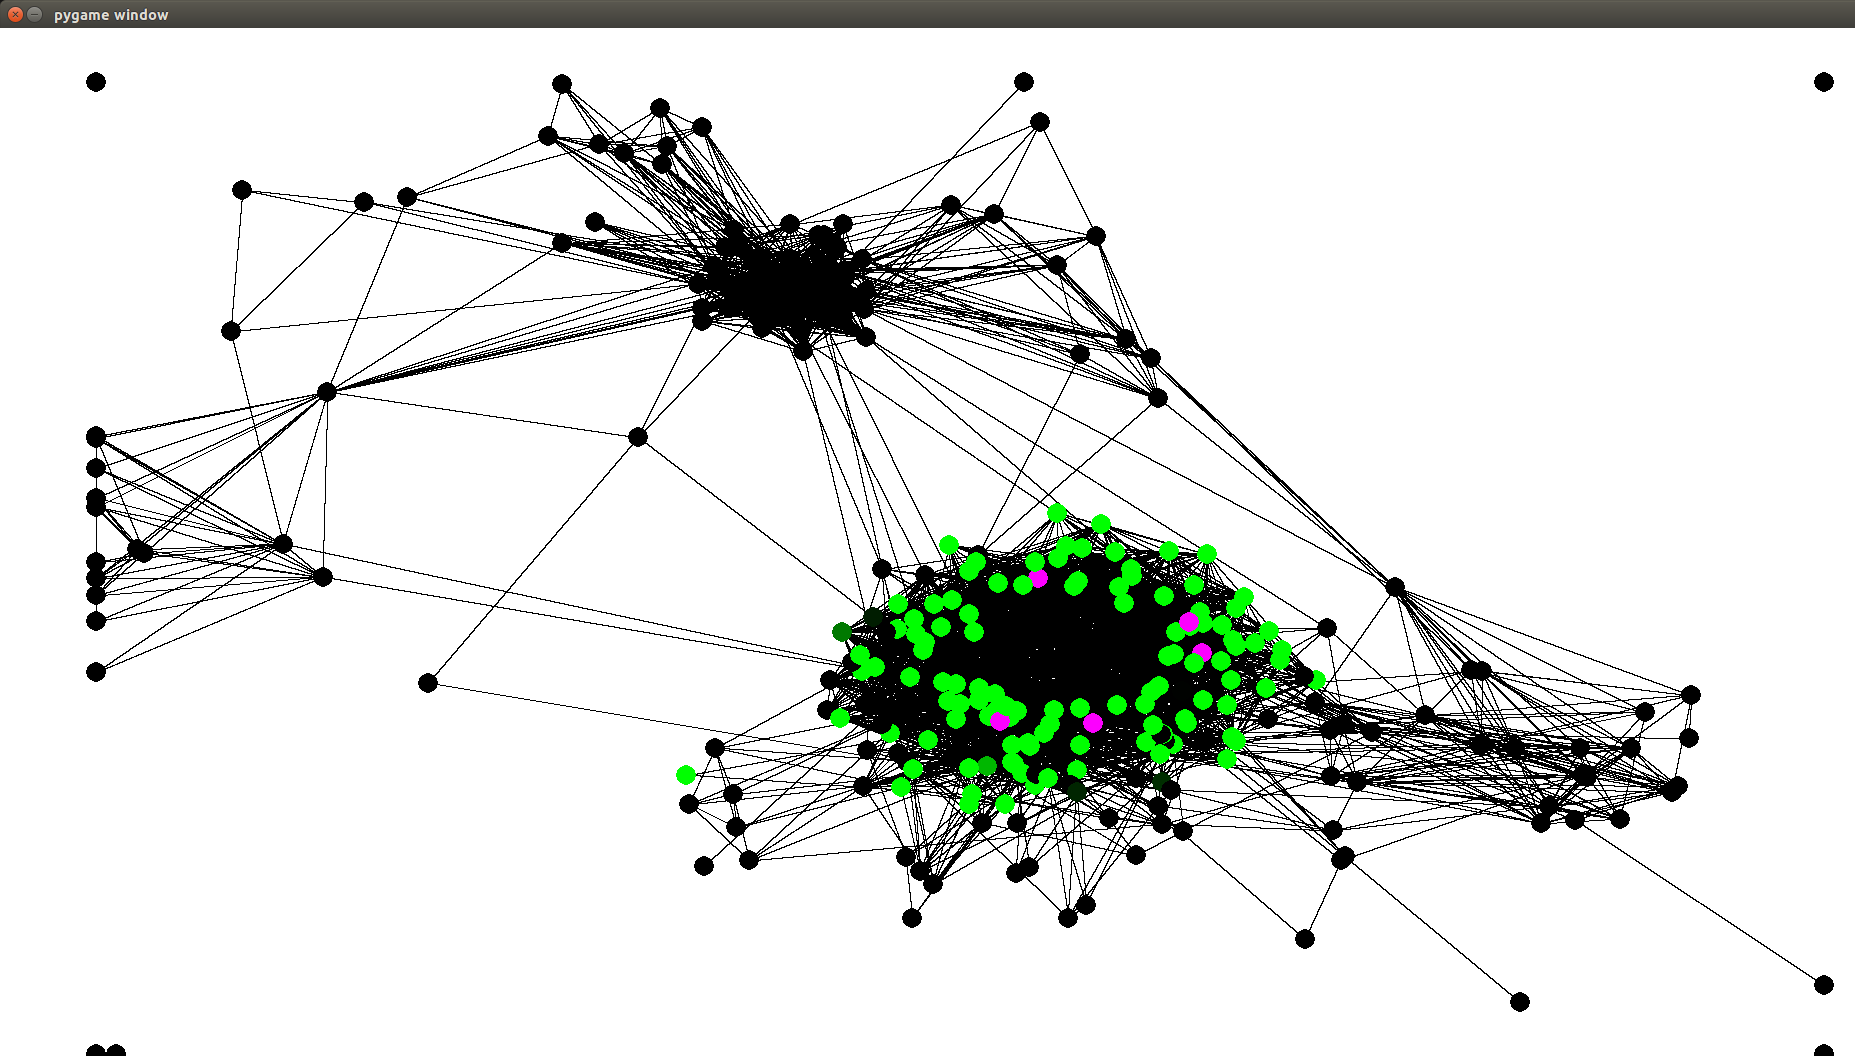
\includegraphics[scale=0.1]{Recommendation1.png}
	\end{subfigure}
\quad
	\begin{subfigure}[b]{0.4\linewidth}
	\caption{View demonstrating everyone's favourite product}
	\label{fig:recommendationFavourite}
	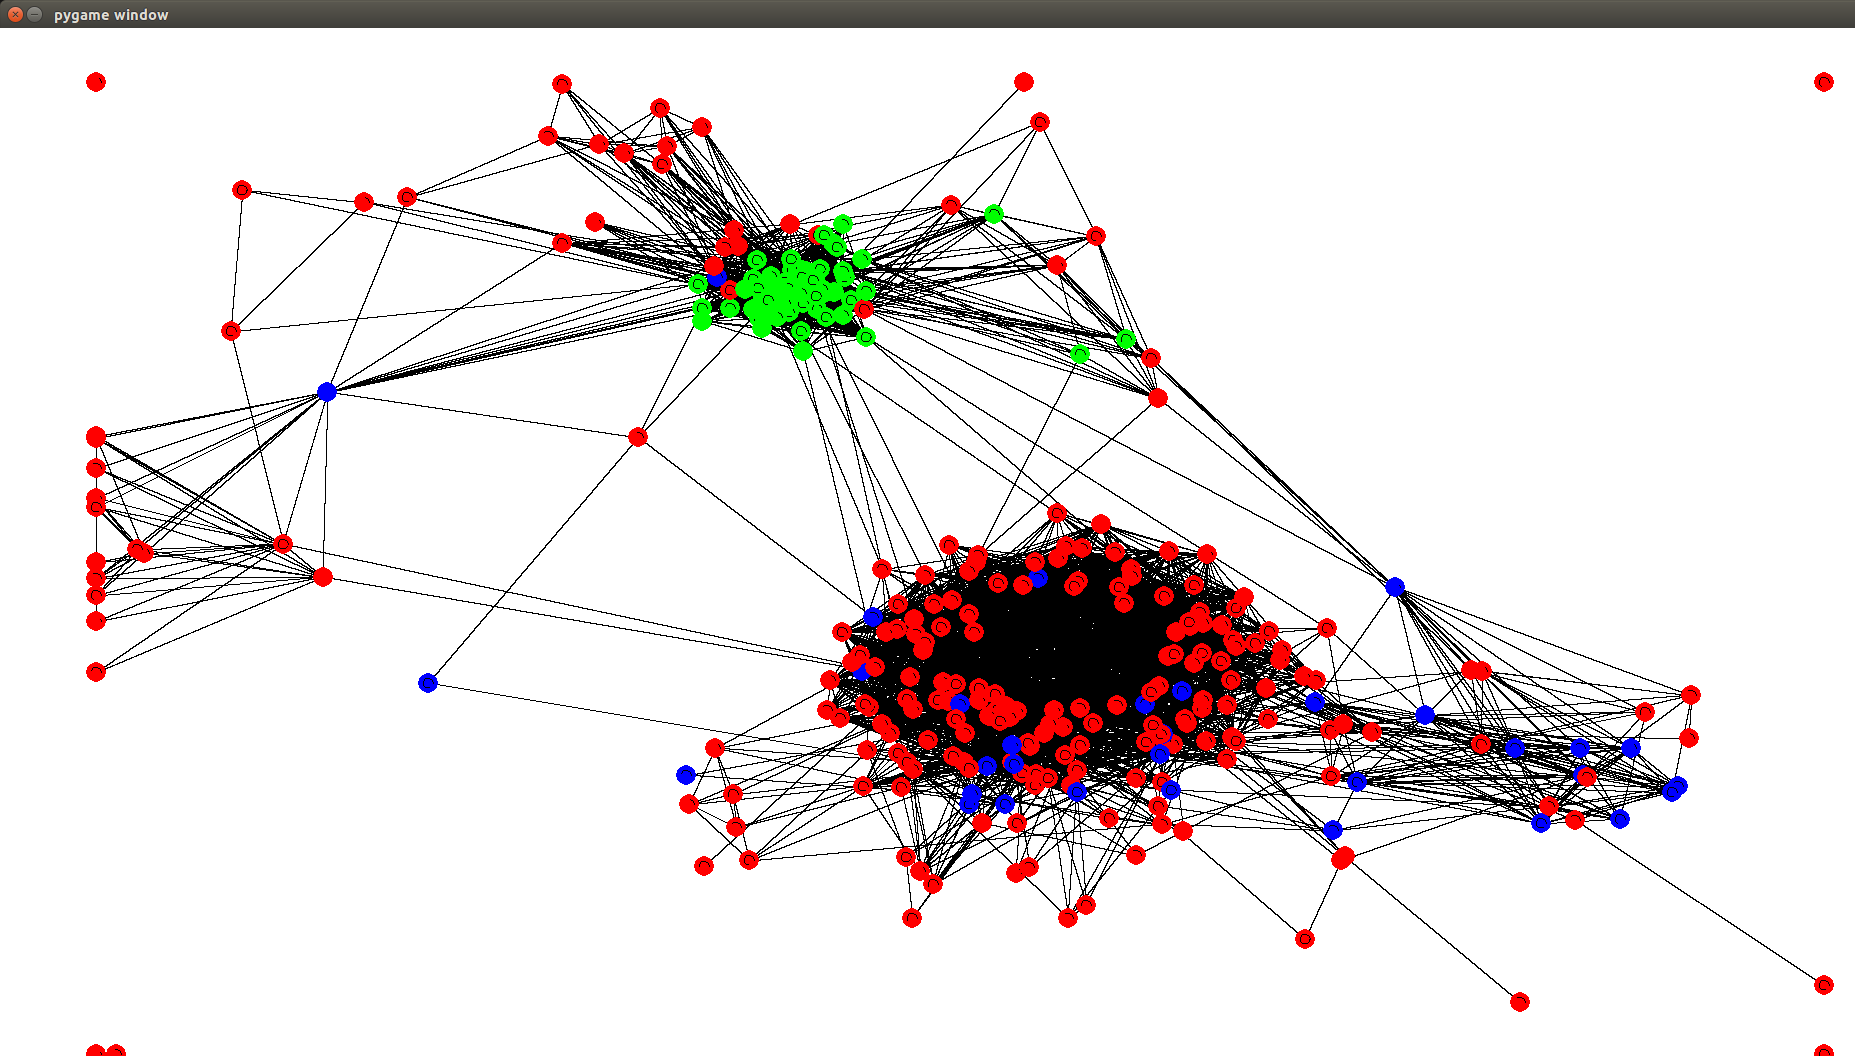
\includegraphics[scale=0.1]{Recommendation2.png}
	\end{subfigure}
	
	\begin{subfigure}[b]{0.4\linewidth}
	\caption{View comparing what products people like}
	\label{fig:RecommendationComparison}
	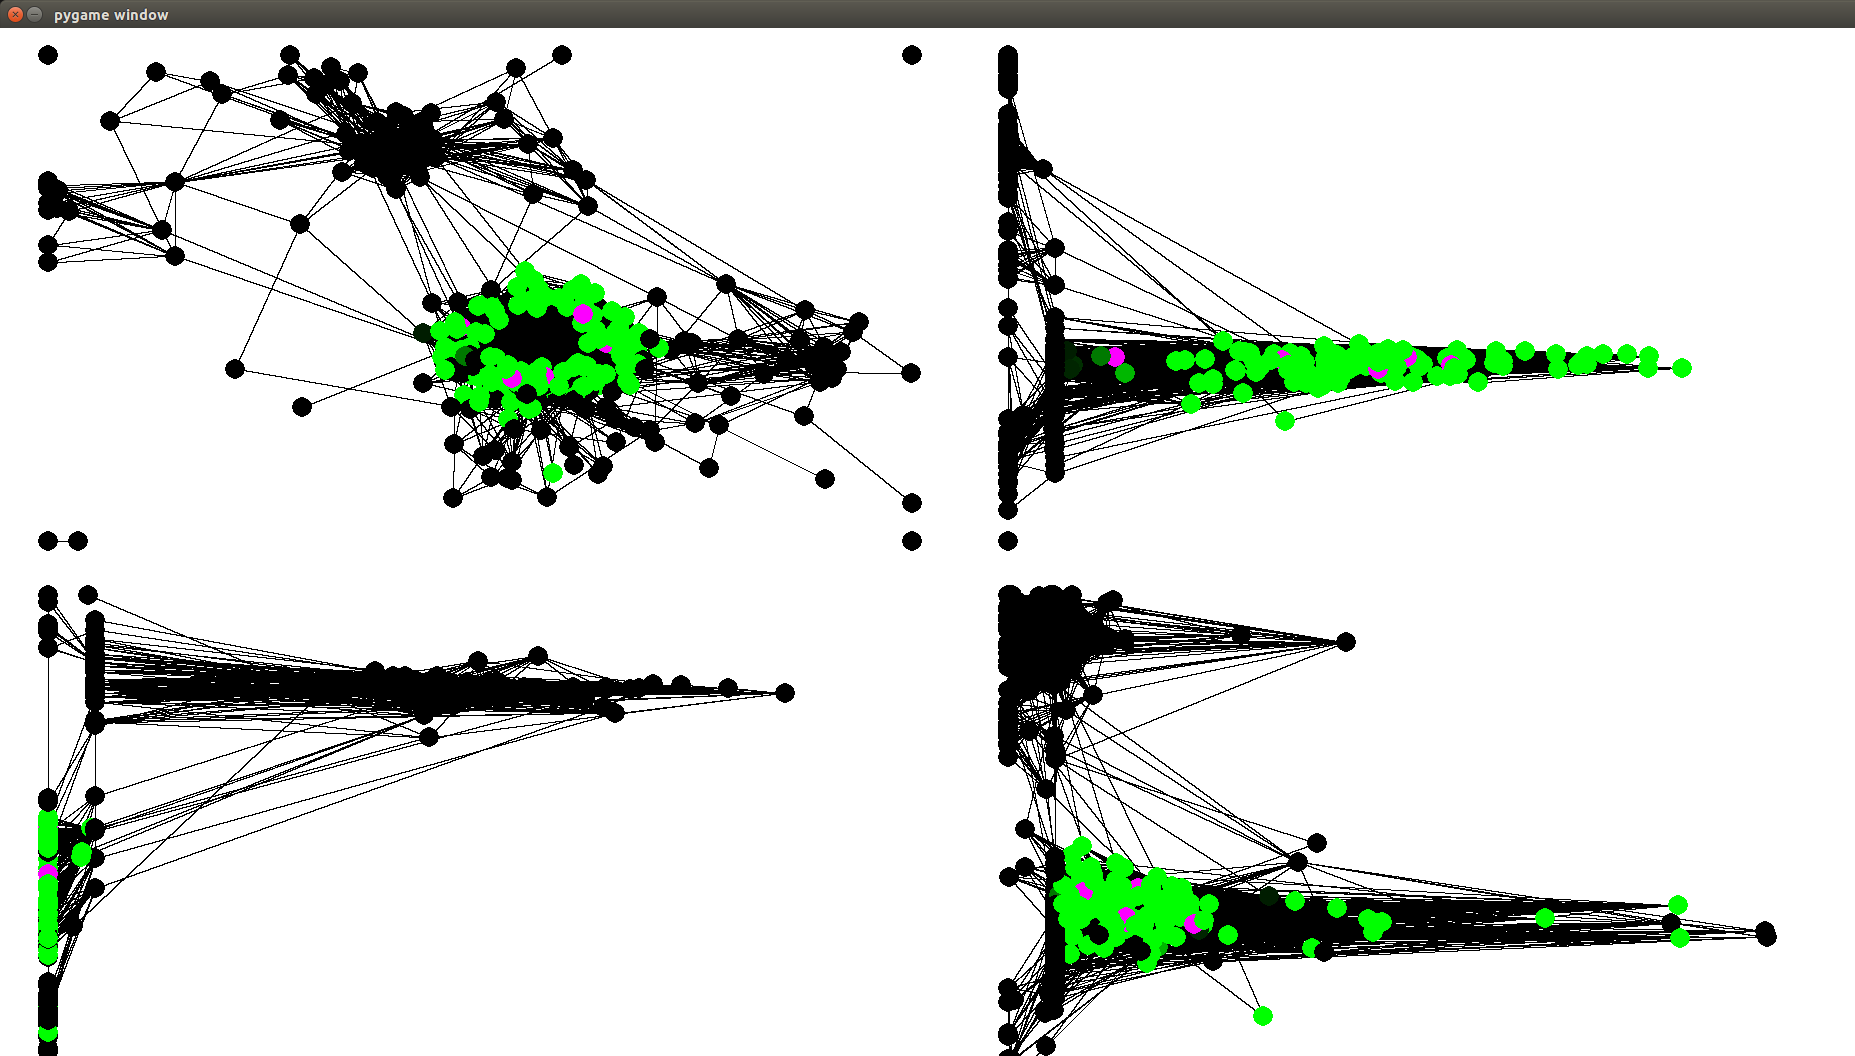
\includegraphics[scale=0.1]{Recommendation3.png}
	\end{subfigure}
\quad
	\begin{subfigure}[b]{0.4\linewidth}
	\caption{View showing different distribution of preerence for another product}
	\label{fig:RecommendationDifferent}
	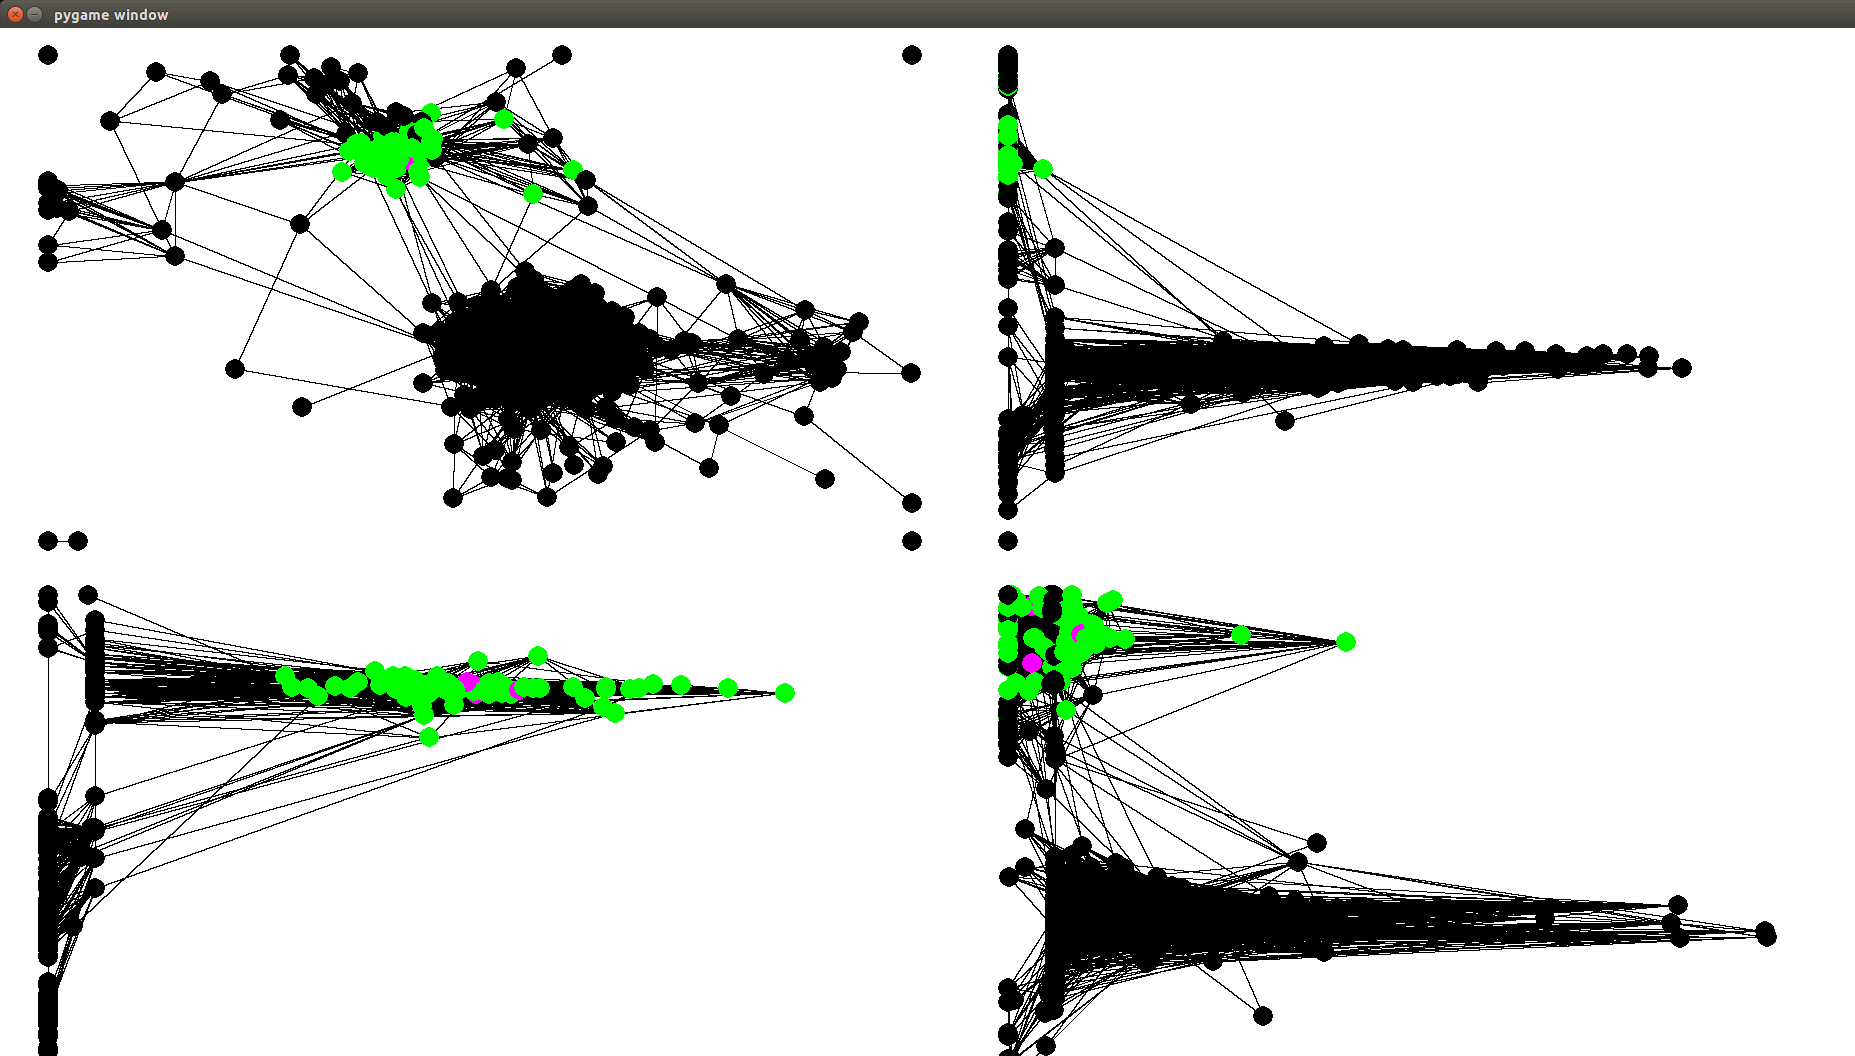
\includegraphics[scale=0.1]{Recommendation4.png}
	\end{subfigure}
\caption{Examples of output produced from the recommendation model}
\label{fig:recommendation}
\end{figure}

\subsection{Influence}

\begin{figure}
\centering
	\begin{subfigure}[b]{0.4\linewidth}
	\caption{Showing selection of vertices to be influenced}
	\label{fig:influenceSelect}
	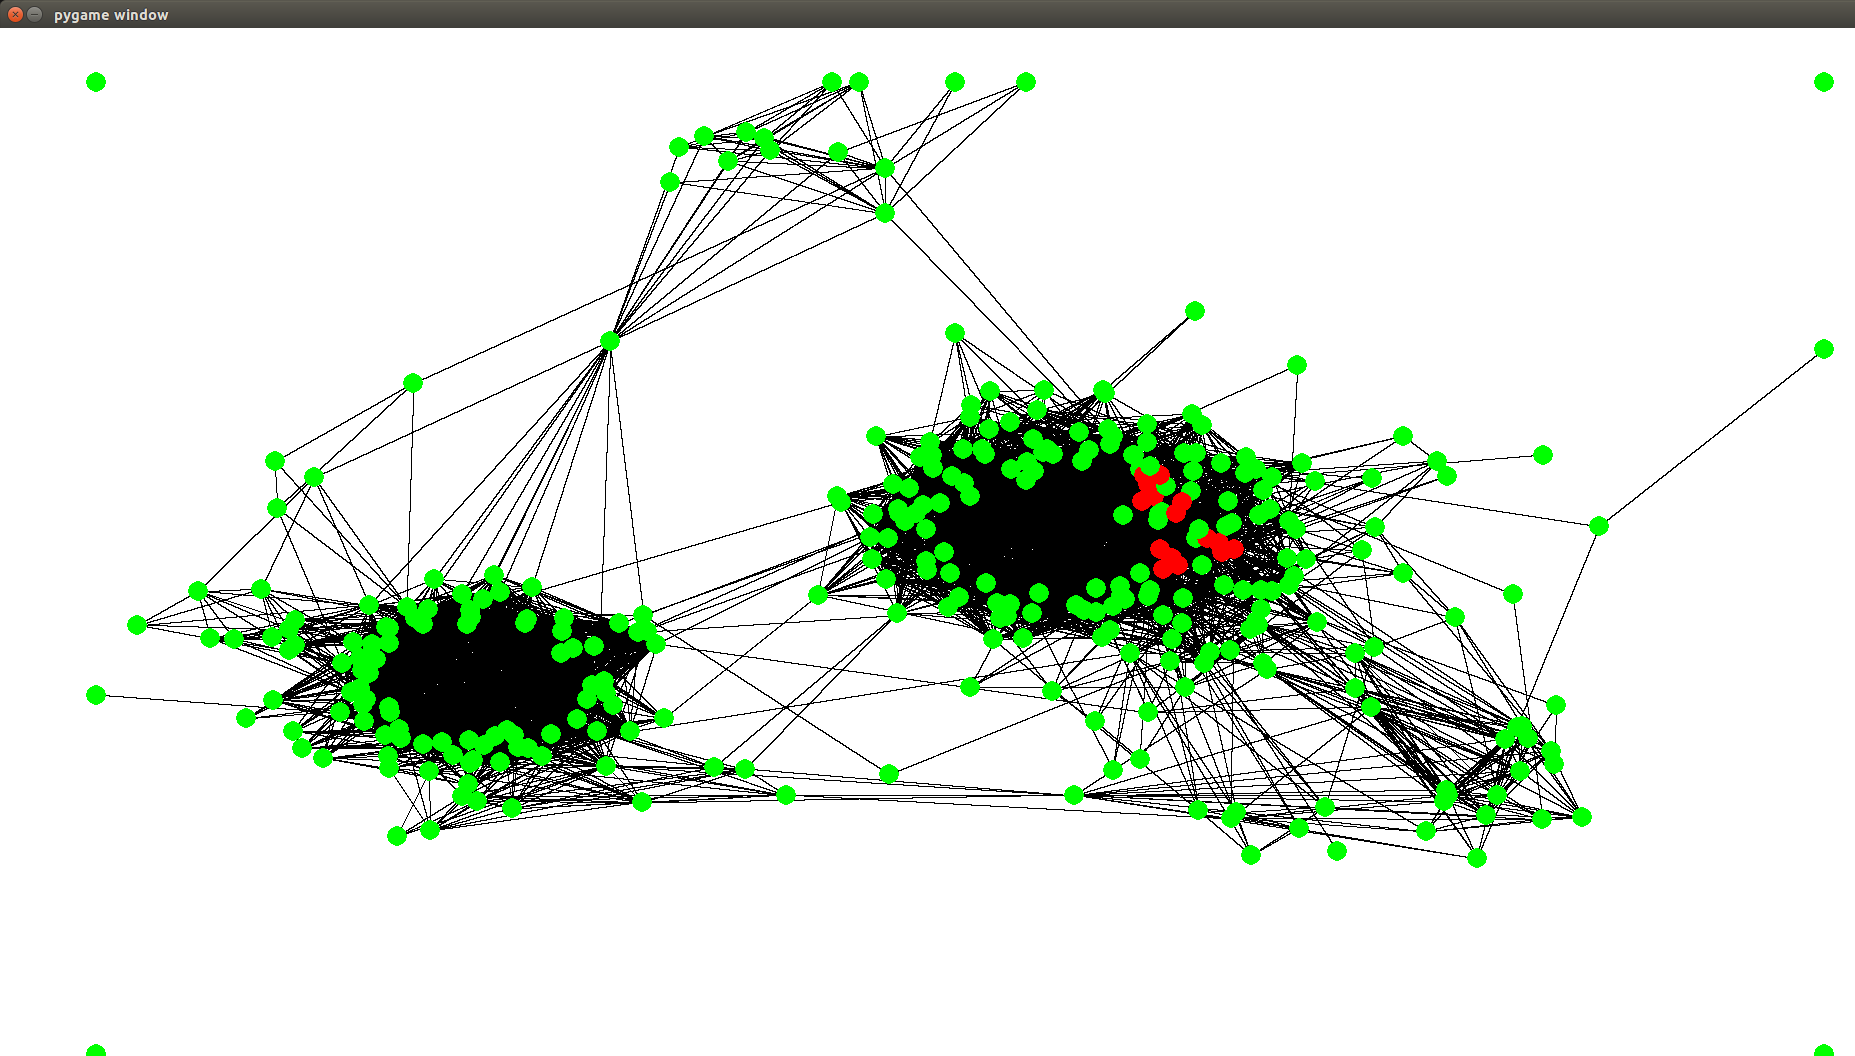
\includegraphics[scale=0.1]{Influence1.png}
	\end{subfigure}
\quad
	\begin{subfigure}[b]{0.4\linewidth}
	\caption{Showing comparison of two models of influence spread}
	\label{fig:influenceCompare}
	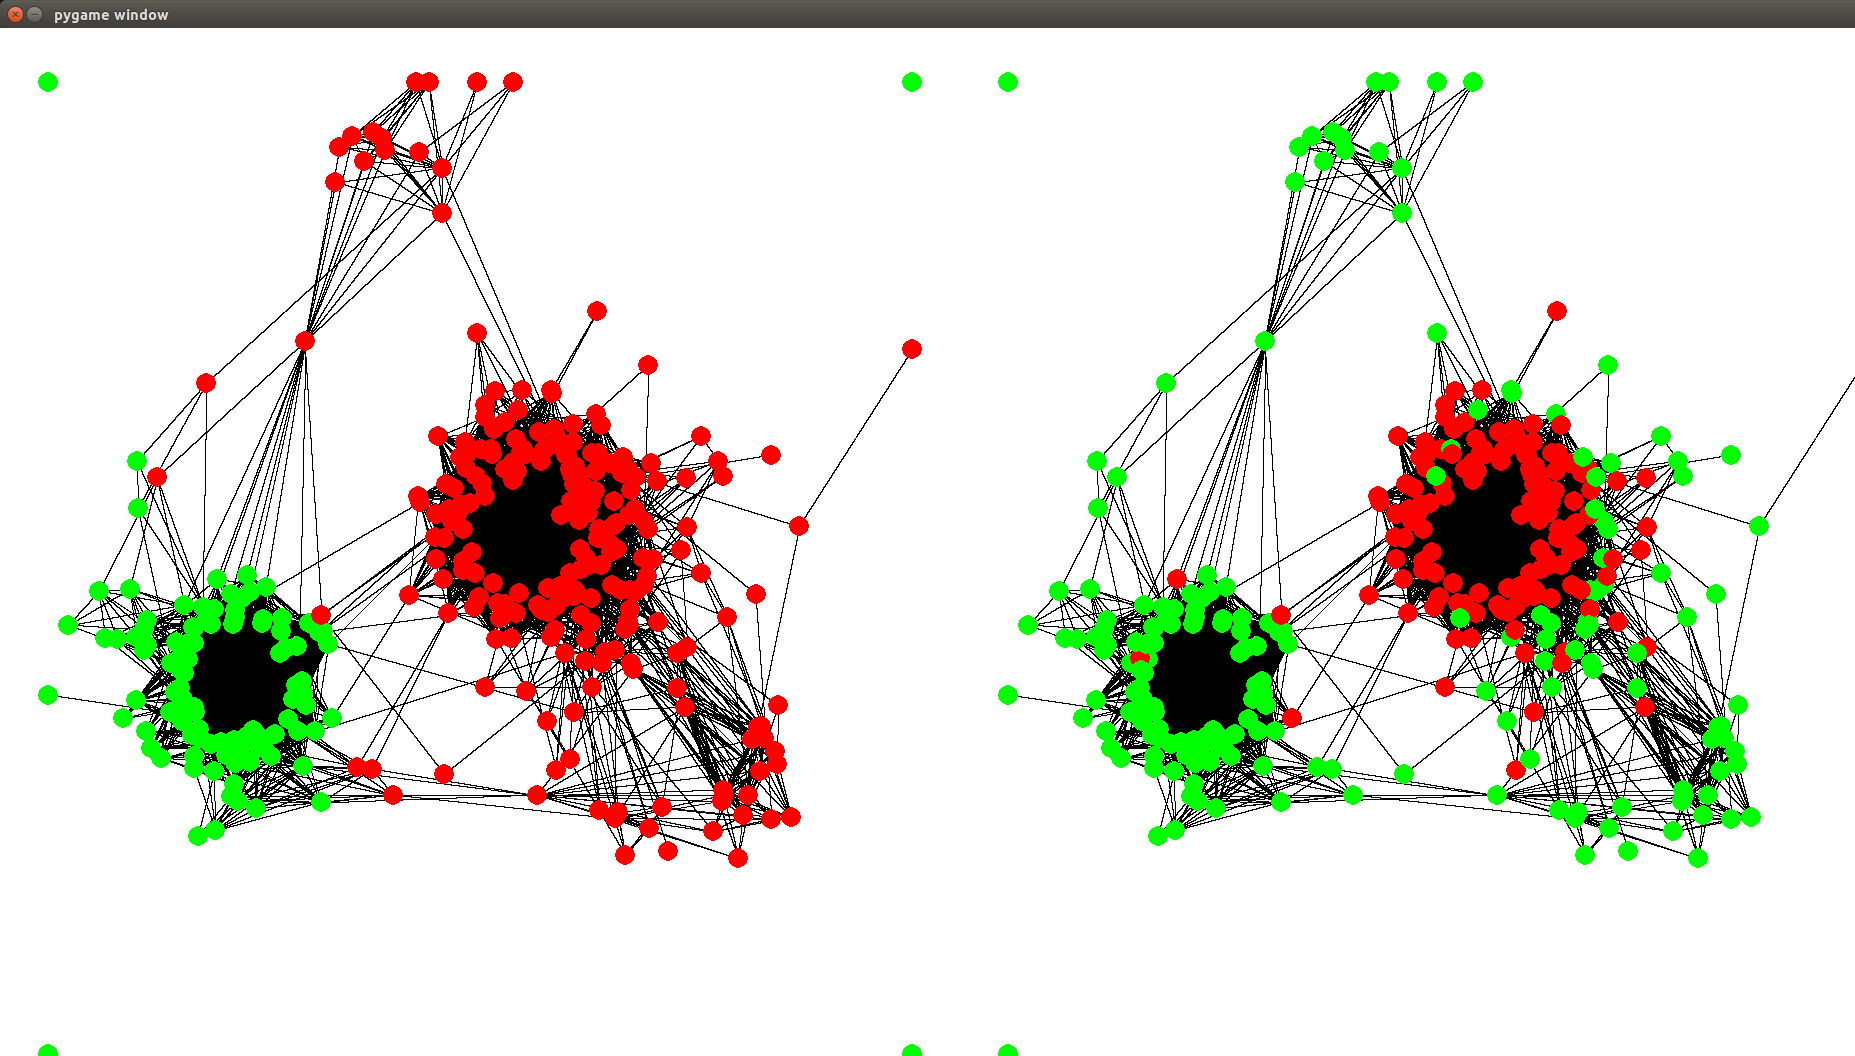
\includegraphics[scale=0.1]{Influence3.png}
	\end{subfigure}
\caption{Example outputs form the influence package}
\label{fig:influence}
\end{figure}

\section{Evaluation}

\section{Conclusions}

\bibliography{projectpaper}


\end{document}